%\documentclass[10pt]{beamer} % aspect ratio 4:3, 128 mm by 96 mm
\documentclass[10pt,aspectratio=169]{beamer} % aspect ratio 16:9

%\graphicspath{{../../figures/}}
\graphicspath{{figs/}{../../figures/}{../../../reports/figures/png/}}
%\includeonlyframes{frame1,frame2,frame3,frame4,frame5,frame6,frame7,frame8,frame9}
%\includeonlyframes{frame10,frame11,frame12,frame13}
%\includeonlyframes{frame14,frame15,frame16,frame17,frame18,frame19,frame20,frame21}
%\includeonlyframes{frame22,frame23,frame24,frame25,frame26}
%\includeonlyframes{frame27,frame28}
%%%%%%%%%%%%%%%%%%%%%%%%%%%%%%%%%%%%%%%%%%%%%%%%%%
% Packages
%%%%%%%%%%%%%%%%%%%%%%%%%%%%%%%%%%%%%%%%%%%%%%%%%%
\usepackage{appendixnumberbeamer}
\usepackage{booktabs}
\usepackage{pgfplots}
\usepackage{xspace}
\usepackage{amsmath}
\usepackage{multirow}
\usepackage{totcount}
\usepackage{tikz}
%\usepackage{comment}
%\usetikzlibrary{external} % speedup compilation
%\tikzexternalize % activate!
%\usetikzlibrary{shapes,arrows}  

%\usepackage{bibentry}
%\nobibliography*
\usepackage{caption}%
\captionsetup[figure]{labelformat=empty}%
%%%%%%%%%%%%%%%%%%%%%%%%%%%%%%%%%%%%%%%%%%%%%%%%%%
% Metropolis theme custom modification file
%%%%%%%%%%%%%%%%%%%%%%%%%%%%%%%%%%%%%%%%%%%%%%%%%%
% Metropolis theme custom modification file
%%%%%%%%%%%%%%%%%%%%%%%%%%%%%%%%%%%%%%%%%%%%%%%%%%
% Metropolis theme custom colors
%%%%%%%%%%%%%%%%%%%%%%%%%%%%%%%%%%%%%%%%%%%%%%%%%%
\usetheme[progressbar=foot]{metropolis}
\useoutertheme{metropolis}
\useinnertheme{metropolis}
\usefonttheme{metropolis}
\setbeamercolor{background canvas}{bg=white}

%\usecolortheme{spruce}

\definecolor{myblue}{rgb}{0.19,0.55,0.91}
\definecolor{mediumblue}{rgb}{0,0,205}
\definecolor{darkblue}{rgb}{0,0,139}
\definecolor{Dodgerblue}{HTML}{1E90FF}
\definecolor{Navy}{HTML}{000080} % {rgb}{0,0,128}
\definecolor{Aliceblue}{HTML}{F0F8FF}
\definecolor{Lightskyblue}{HTML}{87CEFA}
\definecolor{logoblue}{RGB}{1,67,140}
\definecolor{Purple}{HTML}{911146}
\definecolor{Orange}{HTML}{CF4A30}

\setbeamercolor{progress bar}{bg=Lightskyblue}
\setbeamercolor{progress bar}{ fg=logoblue} 
\setbeamercolor{frametitle}{bg=logoblue}
\setbeamercolor{title separator}{fg=logoblue}
\setbeamercolor{block title}{bg=Lightskyblue!30,fg=black}
\setbeamercolor{block body}{bg=Lightskyblue!15,fg=black}
\setbeamercolor{alerted text}{fg=Purple}
%%%%%%%%%%%%%%%%%%%%%%%%%%%%%%%%%%%%%%%%%%%%%%%%%%
%  Theme modifications
%%%%%%%%%%%%%%%%%%%%%%%%%%%%%%%%%%%%%%%%%%%%%%%%%%
% modify progress bar linewidth
\makeatletter
\setlength{\metropolis@progressinheadfoot@linewidth}{2pt} 
\setlength{\metropolis@titleseparator@linewidth}{1pt}
\setlength{\metropolis@progressonsectionpage@linewidth}{1pt}

\setbeamertemplate{progress bar in section page}{
	\setlength{\metropolis@progressonsectionpage}{%
		\textwidth * \ratio{\thesection pt}{\totvalue{totalsection} pt}%
	}%
	\begin{tikzpicture}
	\fill[bg] (0,0) rectangle (\textwidth, \metropolis@progressonsectionpage@linewidth);
	\fill[fg] (0,0) rectangle (\metropolis@progressonsectionpage, \metropolis@progressonsectionpage@linewidth);
	\end{tikzpicture}%
}
\makeatother
\newcounter{totalsection}
\regtotcounter{totalsection}

\AtBeginDocument{%
	\pretocmd{\section}{\refstepcounter{totalsection}}{\typeout{Yes, prepending was successful}}{\typeout{No, prepending was not successful}}%
}%
%%%%%%%%%%%%%%%%%%%%%%%%%%%%%%%%%%%%%%%%%%%%%%%%%%
%  Bibliography mods
%%%%%%%%%%%%%%%%%%%%%%%%%%%%%%%%%%%%%%%%%%%%%%%%%%
\setbeamertemplate{bibliography item}{\insertbiblabel} %% Remove book symbol from references and add number in square brackets
% kill the abominable icon (without number)
%\setbeamertemplate{bibliography item}{}
%\makeatletter
%\renewcommand\@biblabel[1]{#1.} % number only
%\makeatother
% remove line breaks in bibliography
\setbeamertemplate{bibliography entry title}{}
\setbeamertemplate{bibliography entry location}{}
%%%%%%%%%%%%%%%%%%%%%%%%%%%%%%%%%%%%%%%%%%%%%%%%%%
%  Bibliography custom commands
%%%%%%%%%%%%%%%%%%%%%%%%%%%%%%%%%%%%%%%%%%%%%%%%%%
\newcommand{\bibliotitlestyle}[1]{\textbf{#1}\par}

\newif\ifinbiblio
\newcounter{bibkey}
\newenvironment{biblio}[2][long]{%
    %\setbeamertemplate{bibliography item}{\insertbiblabel}
    \setbeamertemplate{bibliography item}{}% without numbers
	\setbeamerfont{bibliography item}{size=\footnotesize}
	\setbeamerfont{bibliography entry author}{size=\footnotesize}
	\setbeamerfont{bibliography entry title}{size=\footnotesize}
	\setbeamerfont{bibliography entry location}{size=\footnotesize}
	\setbeamerfont{bibliography entry note}{size=\footnotesize}
	\ifx!#2!\else%
	\bibliotitlestyle{#2}%
	\fi%
	\begin{thebibliography}{}%
		\inbibliotrue%
		\setbeamertemplate{bibliography entry title}[#1]%
	}{%
		\inbibliofalse%
		\setbeamertemplate{bibliography item}{}%
	\end{thebibliography}%
}

\newcommand{\biblioref}[5][short]{
	\setbeamertemplate{bibliography entry title}[#1]
	\stepcounter{bibkey}%
	\ifinbiblio%
	\bibitem{\thebibkey}%
	#2
	\newblock #4
	\ifx!#5!\else\newblock {\em #5}, #3 \fi%
	\else%
	\begin{biblio}{}
		\bibitem{\thebibkey}
		#2
		\newblock #4
		\ifx!#5!\else\newblock {\em #5}, #3\fi
	\end{biblio}
	\fi
}
%
%\newbibmacro*{hypercite}{%
%	\renewcommand{\@makefntext}[1]{\noindent\normalfont##1}%
%	\footnotetext{%
%		\blxmkbibnote{foot}{%
%			\printtext[labelnumberwidth]{%
%				\printfield{prefixnumber}%
%				\printfield{labelnumber}}%
%			\addspace
%			\fullcite{\thefield{entrykey}}}}}
%
%\DeclareCiteCommand{\hypercite}%
%{\usebibmacro{cite:init}}
%{\usebibmacro{hypercite}}
%{}
%{\usebibmacro{cite:dump}}
%
%% Redefine the \footfullcite command to use the reference number
%\renewcommand{\footfullcite}[1]{\cite{#1}\hypercite{#1}}
%%%%%%%%%%%%%%%%%%%%%%%%%%%%%%%%%%%%%%%%%%%%%%%%%%
% Custom commands
%%%%%%%%%%%%%%%%%%%%%%%%%%%%%%%%%%%%%%%%%%%%%%%%%%
% matrix command 
\newcommand{\matr}[1]{\mathbf{#1}} % bold upright (Elsevier, Springer)
%\newcommand{\matr}[1]{#1}          % pure math version
%\newcommand{\matr}[1]{\bm{#1}}     % ISO complying version
% vector command 
\newcommand{\vect}[1]{\mathbf{#1}} % bold upright (Elsevier, Springer)
% bold symbol
\newcommand{\bs}[1]{\boldsymbol{#1}}
% derivative upright command
\DeclareRobustCommand*{\drv}{\mathop{}\!\mathrm{d}}
\newcommand{\ud}{\mathrm{d}}
% 
\newcommand{\themename}{\textbf{\textsc{metropolis}}\xspace}
%%%%%%%%%%%%%%%%%%%%%%%%%%%%%%%%%%%%%%%%%%%%%%%%%%
%  Title page options
%%%%%%%%%%%%%%%%%%%%%%%%%%%%%%%%%%%%%%%%%%%%%%%%%%
% \date{\today}
\date{}
%%%%%%%%%%%%%%%%%%%%%%%%%%%%%%%%%%%%%%%%%%%%%%%%%%
% option 1
%%%%%%%%%%%%%%%%%%%%%%%%%%%%%%%%%%%%%%%%%%%%%%%%%%
\title{Parametric study of guided wave propagation in honeycomb sandwich panel for model-assisted damage assessment method}
\author{\textbf{Piotr Fiborek}, Pawel Kudela}
% logo align to Institute 
\institute{Institute of Fluid Flow Machinery\\Polish Academy of Sciences \\ \vspace{-1.5cm}\flushright 
\includegraphics[width=4cm]{logo_eng_40mm.eps}}
%%%%%%%%%%%%%%%%%%%%%%%%%%%%%%%%%%%%%%%%%%%%%%%%%%

%%%%%%%%%%%%%%%%%%%%%%%%%%%%%%%%%%%%%%%%%%%%%%%%%%
\begin{document}
%%%%%%%%%%%%%%%%%%%%%%%%%%%%%%%%%%%%%%%%%%%%%%%%%%
\maketitle
\note{Thank you, Mr. Chairman. Good morning everyone. I represent Mechanics of Intelligent Structures Department at the Institute of Fluid Flow Machinery. Today, I am delighted to share our latest research on the numerical modeling of the phenomenon of elastic wave propagation in sandwich panels. The developed model was used to determine the size of damage in the panel.}
%%%%%%%%%%%%%%%%%%%%%%%%%%%%%%%%%%%%%%%%%%%%%%%%%%
% SLIDES
%%%%%%%%%%%%%%%%%%%%%%%%%%%%%%%%%%%%%%%%%%%%%%%%%%
\begin{frame}[label=frame2]{Table of contents \label{frameone}}
  \setbeamertemplate{section in toc}[sections numbered]
  \tableofcontents[hideallsubsections]
  \note{ Here is the outline of my presentation. I will begin with a brief introduction to the subject to set the context for our research. 

  Next, I will describe the model we used in our research. I will explain the basic principles and assumptions of the model.

  This will provide a solid foundation for understanding the methodology we used.

  I will describe our experimental setup to validate the developed model. This validation step is crucial in ensuring the accuracy and reliability of our findings.

  Following that, I will present a method for determining the function that governs the effect of damage size on the propagation of elastic waves. Based on computer simulations, this method allows us to gain valuable insights into the relationship between damage size and wave propagation characteristics. I will then compare the functions obtained from these simulations with the experimental results, highlighting any significant agreements.

  Finally, I will conclude the presentation by summarizing the key points discussed. I will emphasize the contributions and implications of our research and potential future directions.}
\end{frame}
%%%%%%%%%%%%%%%%%%%%%%%%%%%%%%%%%%%%%%%%%%%%%%%%%%
\section{Introduction}
%%%%%%%%%%%%%%%%%%%%%%%%%%%%%%%%%%%%%%%%%%%%%%%%%%
\begin{frame}[label=frame4]{Aim of the research}
\begin{block}{Aim}
	Investigation of guided wave (GW) propagation in honeycomb sandwich composite (HSP) using numerical simulations
\end{block}
\begin{block}{Motivation}
	Assessment of the damage severity in HSP by model-assisted damage identification function (MADIF)
\end{block}
\note{The propagation of elastic waves in Honeycomb Sandwich Panels (HSPs) is a complex phenomenon influenced by their unique construction. Gaining a better understanding of how waves propagate through these panels is crucial for developing effective tools for structural health monitoring. Our motivation is to develop a function that accurately describes the effect of damage size on the characteristic parameters of the propagating wave.}
\end{frame}
\begin{frame}[label=frame6]{Concept of the Method}
\begin{figure}
	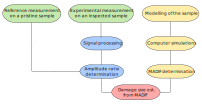
\includegraphics[width=0.9\textwidth]{flowchart.png}
	\caption{A flowchart representing the process for damage size estimation}
\end{figure}
\note{This is a diagram showing the concept of our method leading to the determination of size in the HSP panel. The model is subjected to experimental validation. Then a series of simulations are carried out for different damage sizes, based on which the model assisted damage identification function (MADIF) is obtained.}
\end{frame}


\begin{frame}[label=frame5]{Challenges in modeling of the GW in HSP}
	\footnotesize
	\begin{alertblock}{Challenges}
		\begin{itemize}
			\item complex mesh of the honeycomb core
			\item large number of DOF due to the complexity of the core
			\item large time and memory consuming
		\end{itemize}
	\end{alertblock}
	\begin{columns}
		\column{0.5\textwidth}
	\begin{alertblock}{Most common modeling approaches}
		\begin{itemize}
			\item homogenization of the honeycomb core
			\item reduction of the sample dimensions
			\item simplified model to two-dimensional
			\item omission of an adhesive layer
			\item lack of the transducers
		\end{itemize}
	\end{alertblock}
	\column{0.5\textwidth}
	\begin{alertblock}{Present modeling approach}
	\begin{itemize}
		\item application of fast-convergence numerical methods
		\item parallel computation on the GPU
		\item adhesive layer
		\item incorporate PZT sensors
	\end{itemize}
	\end{alertblock}
	\end{columns}
\note{When attempting to model guided wave (GW) propagation in Honeycomb Sandwich Panels (HSPs), several challenges arise that impact the effectiveness of the simulation. These challenges include the complexity of the core mesh, the large number of degrees of freedom in the model affecting simulation time, and the utilization of operating memory. To address these issues, various techniques have been employed in existing HSP models documented in the literature to enhance efficiency.

	One common approach is the homogenization of material properties, where the core or the entire panel is treated as a homogeneous material. Additionally, the model often incorporates limitations in terms of sample size and the inclusion of specific components such as adhesive layers or sensors.  Additionally, the model is limited in terms of sample size and implemented structure components such as : adhesive layers or sensors.

	In our model, we adopted the spectral element method, recognized as one of the most effective methods for GW modeling. Furthermore, we optimized the algorithm by vectorizing it, enabling parallel calculations on the Graphics Processing Unit (GPU). This approach allowed us to incorporate all the components present in the analyzed sample, thereby enhancing the fidelity of our simulations.}
\end{frame}
%%%%%%%%%%%%%%%%%%%%%%%%%%%%%%%%%%%%%%%%%%%%%%%%%%
\section{Development of the HSP model}
%%%%%%%%%%%%%%%%%%%%%%%%%%%%%%%%%%%%%%%%%%%%%%%%%%
\begin{frame}[label=frame7]{HSP sample configuration}
\begin{table}
	\centering \scriptsize
	\caption{Geometry of HSP [mm]}
	%\begin{tabular}{@{}ccccccc@{}} % remove spaces from vertical lines
	\begin{tabular}{ccccccccccccc} 
		%\hline
		\toprule
		\multicolumn{3}{c}{\textbf{skin}} & {\textbf{adhesive}} & \multicolumn{6}{c}{\textbf{core}} & \multicolumn{2}{c}{\textbf{pzt}} & {\textbf{glue}}\\
		\multicolumn{3}{c}{CFRP $[0^\circ,90^\circ]_s$} & {EA3479B} & \multicolumn{6}{c}{aluminium} & \multicolumn{2}{c}{NCE51} & {CA}\\ 
		%	\hline \hline
		\cmidrule(lr){1-3} \cmidrule(lr){4-4} \cmidrule(lr){5-10} \cmidrule(lr){11-12} \cmidrule(lr){13-13}
		L & W & $g_s$ & $g_a$ & $h_1$ & $h_2$ & $l_1$ & $l_2$ & $g_c$ & $w_c$ & $\Phi$ & $g_t$ & $g_g$\\ 
		%\hline
		%\midrule
		\cmidrule(lr){1-3} \cmidrule(lr){4-4} \cmidrule(lr){5-10} \cmidrule(lr){11-12} \cmidrule(lr){13-13}
		500 & 500 & 1.5 & 0.05 & 11 & 5 & 10.4 & 6 & 14.5 & 0.1 & 10 & 0.5 & 0.05\\
		%\hline 
		\bottomrule 
	\end{tabular} 
	\label{tab:panel_geo}
\end{table}
	\begin{figure}
	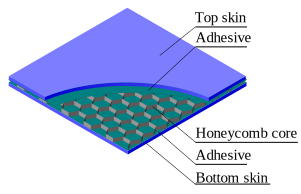
\includegraphics[width=0.75\textwidth]{honeycomb.png}
	\caption{(\textbf{a}) top view of HSP, (\textbf{b}) panel components, (\textbf{c}) details of the honeycomb cell}
	\end{figure}
\note{The object of our research is a sample consisting of carbon skin bonded to aluminium honeycomb.The panel is open on one side so that there is an opportunity to increase the damage. The cell core is a irregular hexagonal with double thickness, from technological point of view, vertical walls.}
\end{frame}

%%%%%%%%%%%%%%%%%%%%%%%%%%%%%%%%%%%%%%%%%%%%%%%%%%
\begin{frame}[label=frame8]{Basis of the Spectral Element Method}
	\begin{itemize}
		\item Division of the domain into non-overlapping finite element
		\item Nodes distribution - endpoints of the element and roots of the first derivative of Legendre polynomial \(\mathcal{P}\) of degree \(p\):
		\begin{equation*}
			(1-\xi^2)\mathcal{P}'_{p}(\xi)=0.
			\label{eq:nodes}
		\end{equation*}
		\item Gauss-Lobatto-Legrendre (GLL) integration scheme:
		\begin{equation*}
			{w(\xi)} = \frac{2}{p(p+1)(\mathcal{P}_{p}(\xi))^2}.
			\label{eq:weight}
		\end{equation*}
		\item Imposing external forces $\textbf{f}_{ext}$ and boundary conditions
		\item Equation of motion:
		\begin{equation*}
			\label{eq:motion}
			\textbf{M} \ddot{\textbf{d}} + \textbf{D} \dot{\textbf{d}} + \textbf{K} \textbf{d} = \textbf{f}_{ext}
		\end{equation*}
		\item Diagonal mass matrix $\textbf{M}$
	\end{itemize}
\end{frame}

\begin{frame}[label=frame11]{Meshes for the components with the interfaces}
	\begin{figure}
		\includegraphics[width=0.78\linewidth]{panel_mesh.png}
		\caption{The meshes of HSP components and the interfaces}
		\label{fig:panel_mesh}
	\end{figure}
\end{frame}
\begin{frame}[label=frame12]{Disbonds models}
	\begin{figure}
		\includegraphics[width=1\linewidth]{disbond.png}
		\caption{The damaged area in the: (\textbf{a}) experimental sample, (\textbf{b}) numerical model with removed cells and (\textbf{c}) numerical model with interface decoupling}
		\label{fig:disbonds}
	\end{figure}
\end{frame}
\begin{frame}[label=frame11]{Models comparison}
\begin{figure}
	\includegraphics[width=1\linewidth]{figs/fullfield_100_0}
	\label{fig:fulfield_100kHz_0}
\end{figure}
\end{frame}
\section{Experimental Validation of the Method }
%%%%%%%%%%%%%%%%%%%%%%%%%%%%%%%%%%%%%%%%%%%%%%%%%%
\begin{frame}[label=frame13]{Experimental validation setup}
	\begin{columns}[T]
		\column{0.55\textwidth}
	\begin{figure}
		\includegraphics[width=0.7\linewidth]{pzt_setup.png}
		\footnotesize
		\caption{(\textbf{a}) the wave generation/acquisition setup: DMU - the data management unit, G1, G2 - the arbitrary wave generator, O - the oscilloscope, HVA - the voltage amplifier, LWDS - the Lamb Wave Detection Systems, (\textbf{b}) the specimen with PZTs}
		\label{fig:pzt_setup}
	\end{figure}
		\column{0.45\textwidth}
		\begin{figure}
			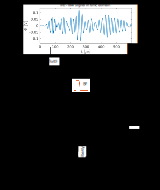
\includegraphics[width=0.8\linewidth]{signal_processing.png}
			\caption{Flowchart for signal processing}
			\label{fig:signal_processing}
		\end{figure}
	\end{columns}	
\end{frame}
\begin{frame}[label=frame14]{Experimental validation results - single skin plate}
		\begin{figure}
			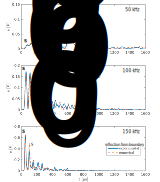
\includegraphics[width=1\linewidth]{single_skin.png}
			\label{fig:single_skin}
		\end{figure}
\end{frame}

\begin{frame}[label=frame15]{Experimental validation results - single CFRP}
	\begin{table}
		\centering
		\caption{\label{tab:group_velocity_cfrp} Comparison between amplitudes and group velocities obtained from the simulations and experiments for single skin plate}
		\begin{tabular}{cccccccc}
			\toprule
			& & \multicolumn{3}{c}{\(C_g\)} & \multicolumn{3}{c}{Amp.}\\
			Mode & Frequency & Exp. & Num. & \(\delta\)& Exp. & Num. & \(\delta\)\\
			& kHz & m/s & m/s & \% & mV & mV & \% \\
			\midrule
			\multirow{3}{*}{$S_0$} & 50 & 6079 & 5865 & \textcolor{green}{3.52}& 12 & 171 & \textcolor{red}{25.0} \\
			&100& 5571 & 5747 & \textcolor{green}{3.16} & 171 & 162 & \textcolor{green}{5.26}\\
			&150& 5764 & 5698 & \textcolor{green}{1.15} & 648 & 664 & \textcolor{green}{2.47}\\
			\midrule
			\multirow{3}{*}{$A_0$} &50& 1341 & 1325 & \textcolor{green}{0.74} & 134 & 125 & \textcolor{green}{6.72}\\
			&100& 1550 & 1396 & \textcolor{green}{9.74} & 84 & 104 & \textcolor{red}{23.8}\\
			\bottomrule
		\end{tabular}
	\end{table}
\end{frame}
\begin{frame}[label=frame15]{Experimental validation results - HSP based on the full core geometry model (\textbf{FCGM}) }
	\begin{figure}
			\includegraphics[width=1\linewidth]{HSP_full.png}
			\label{fig:HSP_full}
		\end{figure}
\end{frame}
\begin{frame}[label=frame16]{Experimental validation results - HSP}
	\begin{table}
		\centering
		\caption{\label{tab:group_velocity_hsp} Comparison between amplitudes and group velocities obtained from the simulations based on the FCGM and experiments for HSP}
		\begin{tabular}{cccccccc}
			\toprule
			& & \multicolumn{3}{c}{\(C_g\)} & \multicolumn{3}{c}{Amp.}\\
			Mode & Freq. & Exp. & FCGM & \(\delta\) & Exp. & FCGM & \(\delta\)\\
			& kHz & m/s & m/s & \% & mV & mV & \%\\
			\midrule
			\multirow{3}{*}{$S_0$} & 50 & 6452 & 8696 & {34.78}& 32 & 6 & \textcolor{red}{81.25}\\
			&100& 5263 & 5128 & \textcolor{green}{2.57}& 369 & 314 & \textcolor{green}{14.91}\\
			&150& 5085 & 5217 & \textcolor{green}{2.60}& 1341 & 1239 & \textcolor{green}{7.61}\\
			\midrule
			\multirow{2}{*}{$A_0$} & 50 & 966 & 926 & \textcolor{green}{4.14} & 1316& 76 & {22.58}\\
			& 100 & 2174 & 2151 & \textcolor{green}{1.06} & 137 & 179 & {30.66}\\
			\bottomrule
		\end{tabular}
	\end{table}
\end{frame}
\section{Model-Assisted Damage Identification Function}
%%%%%%%%%%%%%%%%%%%%%%%%%%%%%%%%%%%%%%%%%%%%%%%%%%
\begin{frame}[label=frame17]{Model-Assisted Damage Identification Function (MADIF)}
\begin{figure}
	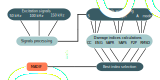
\includegraphics[width=1\linewidth]{madif_extract.png}
	\label{fig:madif_ectract}
\end{figure}
\end{frame}

\begin{frame}[label=frame21]{MADIF determination - full length 100 kHz signal}
		
		\begin{columns}[T]
			\column{0.4\textwidth}
			\begin{block}{MADIF determination}
				\begin{itemize}
					\item Fitting functions:\\
					\footnotesize
					\begin{equation*}
						f_1(x) = \frac{a_2x}{(x+a_1)}+a_0
						\label{eq:f1}
					\end{equation*}
					\begin{equation*}
						f_2(x) = a_2\sqrt{x}+a_1x +a_0
						\label{eq:f2}
					\end{equation*}
					\begin{equation*}
						f_3(x) = \frac{a_3x}{\sqrt{a_2x^2+a_1}}+a_0
						\label{eq:f3}
					\end{equation*}
				\end{itemize}
					\begin{itemize}
						\item Mean absolute error:\\
						\footnotesize
						\begin{equation*}
							\delta^{\mathrm{fit}} = \frac{1}{\mathrm{n^{DI}}}\sum_{i=1}^{\mathrm{n^{DI}}} \left|\frac{\mathrm{DI^i_{n}}-f(x^i)}{\mathrm{DI^i_{n}}}\right|\times100
							\label{eq:delta}
						\end{equation*}
					\end{itemize}
				\end{block}
				\column{0.6\textwidth}
				\begin{figure}
					\includegraphics[width=1\linewidth]{RMSD.png}
					\label{fig:RMSD_full_100}
				\end{figure}
			\end{columns}

\end{frame}

\begin{frame}[label=frame22]{MADIF vs. experimental results}
	\begin{block}{MADIF based on RMSD for full length 100 kHz signal with interface removed model}
		\footnotesize
		\begin{equation*}
			\mathrm{MADIF}^\mathrm{RMSD} = \frac{13.44w_d}{(w_d+38.12)}+0.64
			\label{eq:rmsd}
		\end{equation*}
	\end{block}
\begin{figure}
	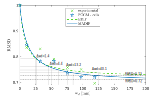
\includegraphics[width=0.8\linewidth]{MADIF_RMSD.png}
	\label{fig:MADIF_RMSD}
\end{figure}
\end{frame}
%%%%%%%%%%%%%%%%%%%%%%%%%%%%%%%%%%%%%%%%%%%%%%%%%%%%%%%%%%%%%%%%%%%%%%%%%%%%%%%%%%
\section{Parametric study}
\begin{frame}[label=frame24]{The temperature depending material properties}
	\begin{figure}
		\includegraphics[width=1\linewidth]{skin_temp.png}
		\label{fig:SKIN_TEMP}
	\end{figure}
\end{frame}

\begin{frame}[label=frame24]{The temperature depending material properties - PZT}
	\begin{figure}
		\includegraphics[width=1\linewidth]{pzt_temp.png}
		\label{fig:PZT_TEMP}
	\end{figure}
\end{frame}

\begin{frame}[label=frame24]{The temperature depending MADIF - RMSD}
	\begin{figure}
		\includegraphics[width=1\linewidth]{MADIF_RMSD_TEMP.png}
		\label{fig:MADIF_RMSD_TEMP}
	\end{figure}
\end{frame}

\begin{frame}[label=frame25]{Simply supported \& clamped BC}
	\begin{figure}
		\includegraphics[width=1\linewidth]{panel_BC.png}
		\label{fig:panel_BC}
	\end{figure}
\end{frame}

\begin{frame}[label=frame25]{MADIF for various boundary conditions }
	\begin{figure}
		\includegraphics[width=1\linewidth]{MADIF_BC.png}
		\label{fig:MADIF_CC_BC}
	\end{figure}
\end{frame}

\begin{frame}[label=frame25]{Effect of the PZT parameters on GW propagation}
	\begin{figure}
		\begin{center}
			\includegraphics[width=0.5\textwidth]{pzt_place}
		\end{center}
		\caption{The GW propagation in the HSP (\textbf{a}), sensor responses for (\textbf{b}) different PZT placement in relation to the core cell}
		\label{fig:pzt_place}
	\end{figure}
\end{frame}

\begin{frame}[label=frame25]{Effect of the PZT parameters on GW propagation}
	\begin{figure}
		\begin{center}
			\includegraphics[width=0.8\textwidth]{pzt_eps}
		\end{center}
		\caption{The signal envelopes for \textbf{the piezoelectric dielectric permittivity} in the range of 80\%-120\% of the reference value}
		\label{fig:pzt_eps}
	\end{figure}
\end{frame}

\begin{frame}[label=frame25]{Effect of the core parameters on GW propagation}
	\begin{figure}
		\begin{center}
			\includegraphics[width=0.8\textwidth]{core_size}
		\end{center}
		\caption{The signal envelopes for the various \textbf{the core size} in the range 5.0-9.0 mm}
		\label{fig:core_size}
	\end{figure}
\end{frame}

\begin{frame}[label=frame25]{Effect of the core parameters on GW propagation}
	\begin{figure}
		\begin{center}
			\includegraphics[width=0.8\textwidth]{core_height}
		\end{center}
		\caption{The signal envelopes for the various \textbf{core heights} in the range 10.5-18.5 mm}
		\label{fig:core_height}
	\end{figure}
\end{frame}

%%%%%%%%%%%%%%%%%%%%%%%%%%%%%%%%%%%%%%%%%%%%%%%%%%%%%%%%%%%%%%%%%%%%%%%%%%%%%%%%%%%
\section{Final remarks}
\begin{frame}[label=frame24]{Final remarks}
	\begin{alertblock}{Conclusions}
		\begin{itemize}
			\item development of the full core geometry model based on the spectral element method
			\item determination of the model-assisted damage identification function for honeycomb sandwich panel
			\item excellent agreement the MADIF with the experimental results
		\end{itemize}
	\end{alertblock}
\begin{alertblock}{Future works}
	\begin{itemize}
		\item analyzing the functions for damage with different shapes and various localization
		\item develop HSP material properties optimization tool
	\end{itemize}
\end{alertblock}
\end{frame}
{\setbeamercolor{palette primary}{fg=black, bg=white}
	\begin{frame}[standout]
		Thank you for your attention!\\ \vspace{12pt}
		\scriptsize{\url{pfiborek@imp.gda.pl}}
		\begin{block}{Acknowledgement}
			\tiny
			Author would like to gratefully acknowledge the support given by the National Science, Poland under agreement no. 2018/31/N/ST8/02865 in the frame of PRELUDIUM project entitled: 'Model-assisted damage identification function for Structural Health Monitoring of composite structures under a varied environmental condition'
			\begin{figure}
				\includegraphics[width=0.25\linewidth]{NCN.png}
				\label{fig:NCN}
			\end{figure}
		\end{block}
	\end{frame}
}
\end{document}